%xelatex
\documentclass{article}
\usepackage[margin=0.6in]{geometry}
\usepackage{xltxtra}
\usepackage{xgreek}
\usepackage{listing}
\setmainfont[Mapping=tex-text]{Kerkis}
\usepackage[colorlinks=true,linkcolor=black,urlcolor=blue]{hyperref}
\title{Παράλληλη επεξεργασία}
\author{Μπαντολας Πέτρος 5028\\Σειμένης Σπύρος 5070\\Καλλιβωκάς Δημήτριος 4993}

\begin{document}
\maketitle
\section{Ανάλυση σειριακής έκδοσης}
- ΑΝΑΛΥΣΗ ΤΟΥ ΚΩΔΙΚΑ ΜΕ ΧΡΗΣΗ SCALASCA\\
- SCREENSHOT ΑΠΟ SCALASCA
- ..

\section{Παραλληλοποίηση}
\subsection{Με χρήση OpenMP}
-ΑΙΤΙΟΛΟΓΗΣΗ ΠΑΡΑΛΛΗΛΟΠΟΙΗΣΗΣ
-ΜΕΤΡΗΣΕΙΣ

\subsection{Με χρήση εντολών SIMD}
-ΑΙΤΙΟΛΟΓΗΣΗ ΒΕΛΤΙΣΤΟΠΟΙΗΣΗΣ
-ΜΕΤΡΗΣΕΙΣ






\end{document}



%\begin{center}
%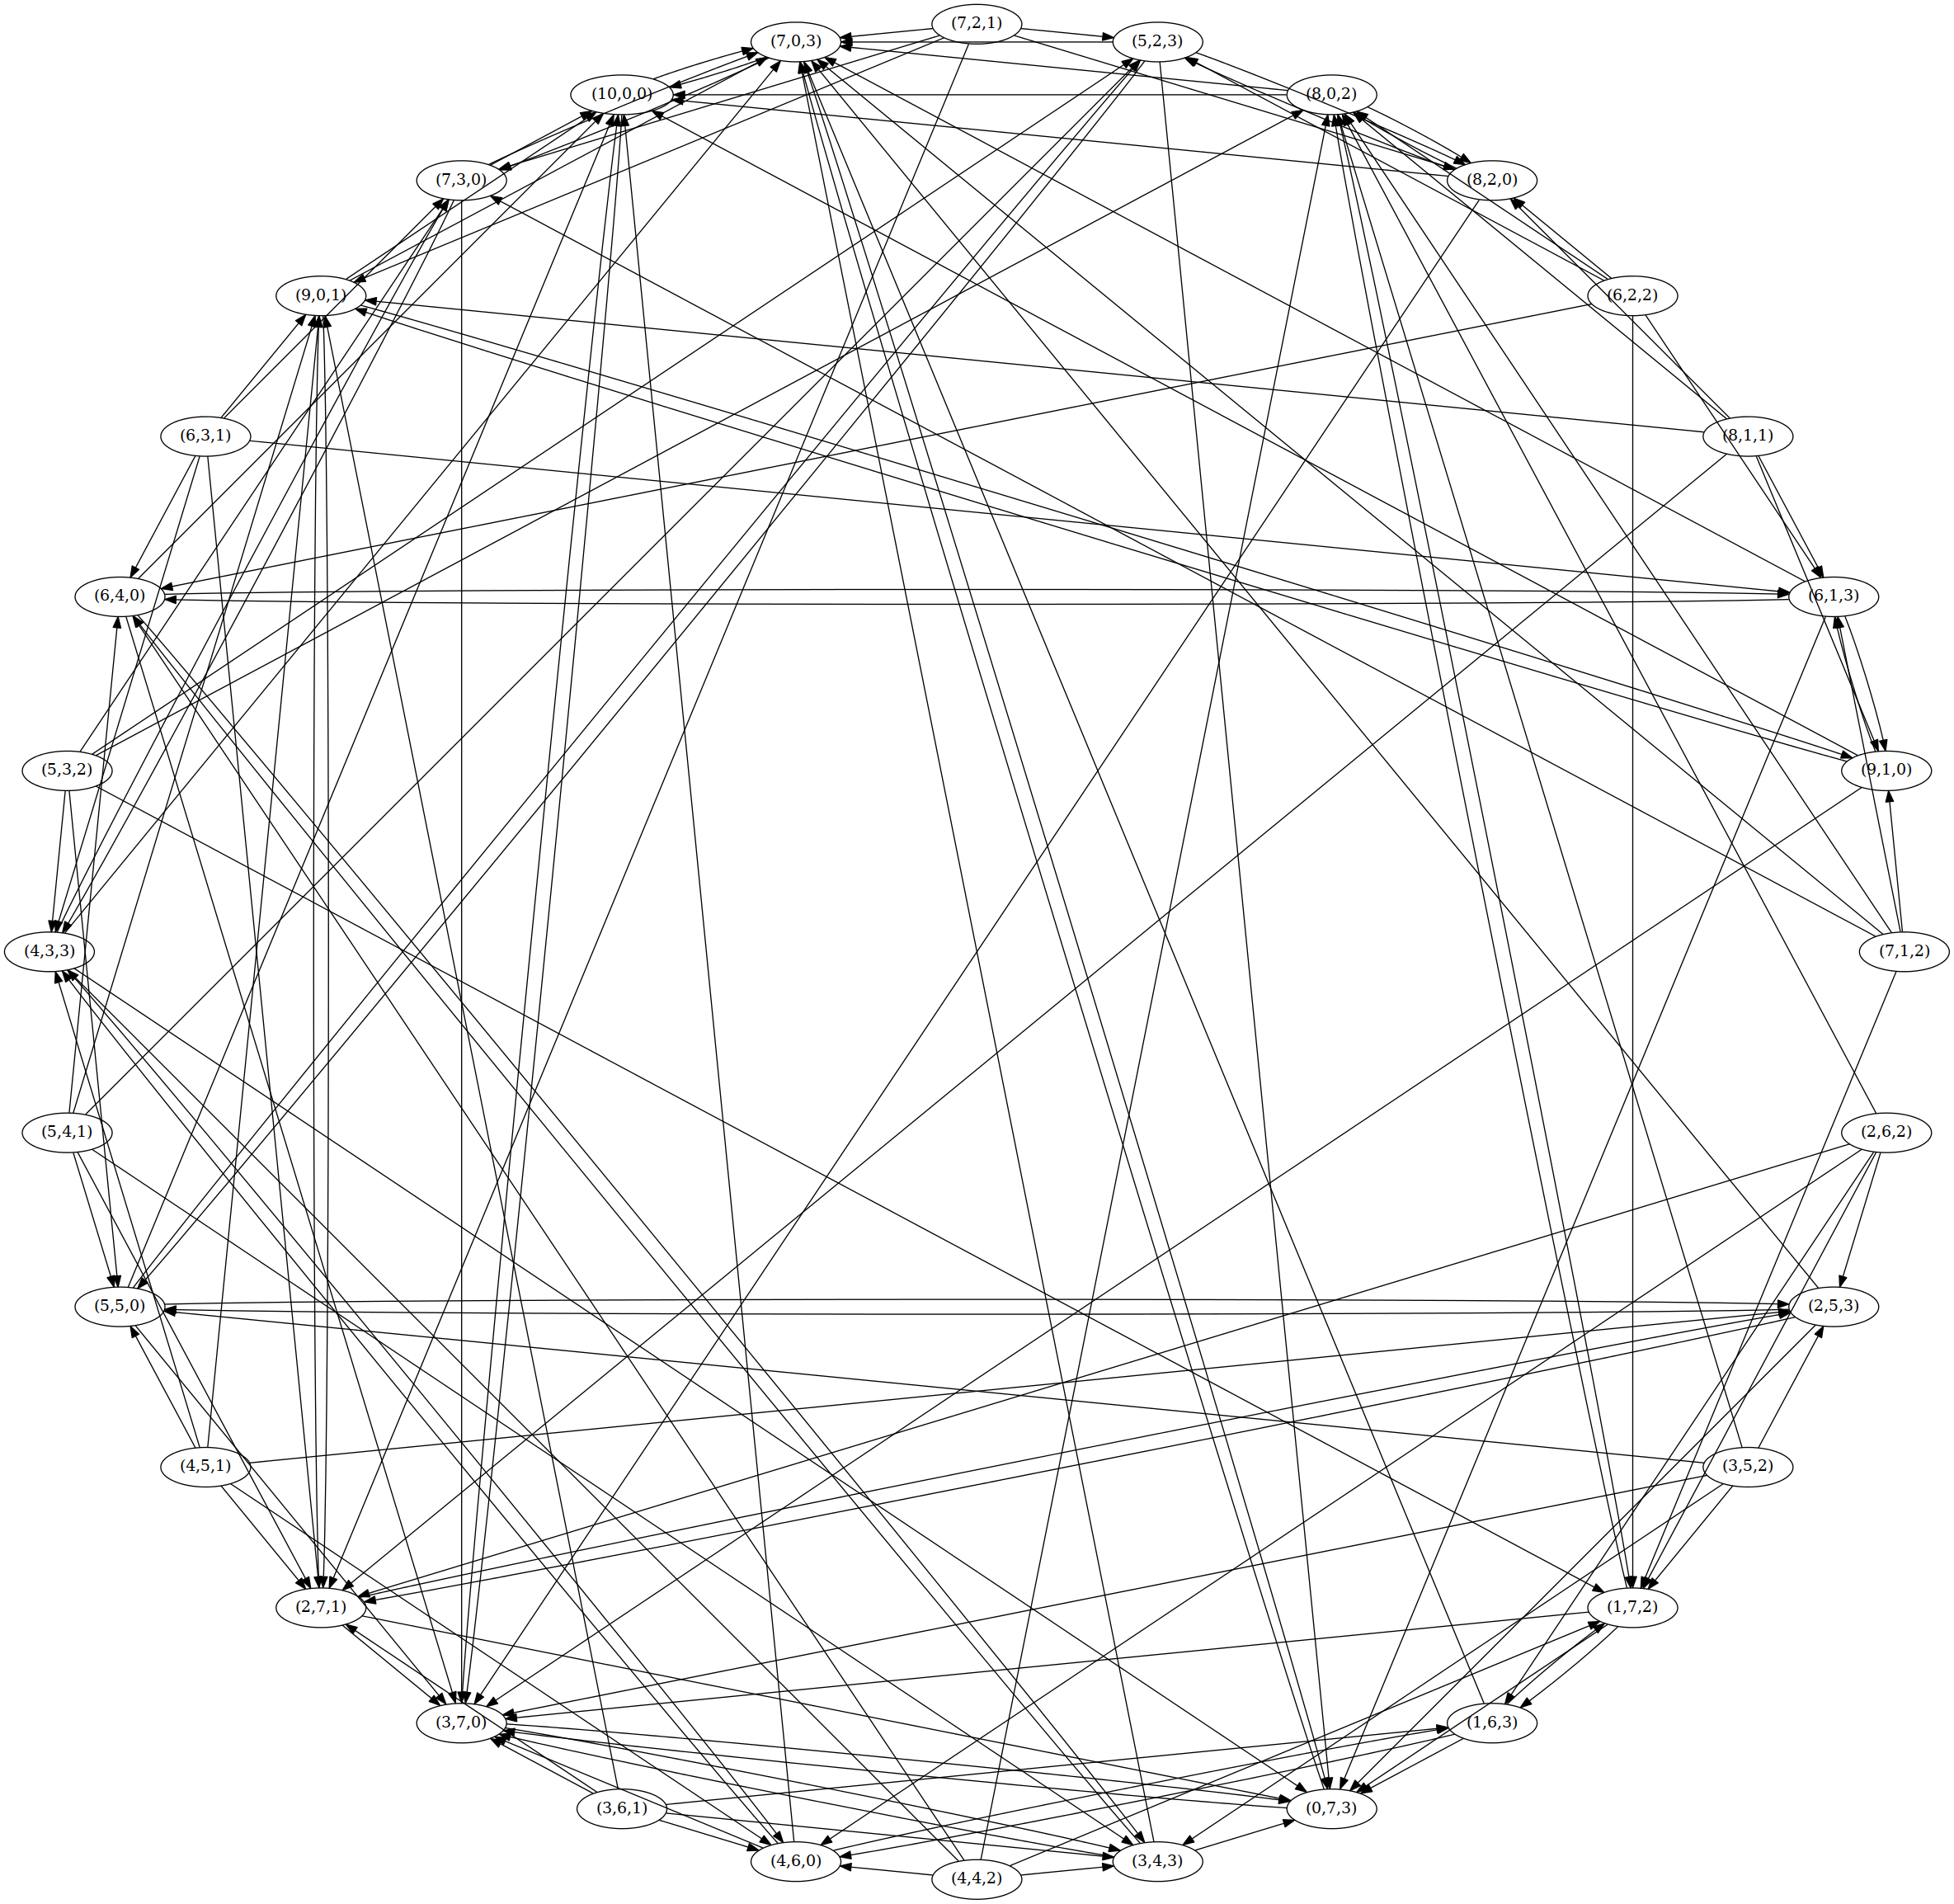
\includegraphics[scale=0.18]{../graph.png}
 % graph.png: 2369x2308 pixel, 300dpi, 20.06x19.54 cm, bb=0 0 569 554
%\end{center} 